% Capitolul 9: Prophet și TBATS
% Prezentare academică de calitate Harvard
% Program de licență, Academia de Studii Economice din București

\documentclass[9pt, aspectratio=169, t]{beamer}

% Asigură încadrarea conținutului pe diapozitive
\setbeamersize{text margin left=8mm, text margin right=8mm}

%=============================================================================
% CONFIGURARE TEMĂ ȘI STIL
%=============================================================================
\usetheme{default}
% Using default theme for clean header/footer control

% Color Palette (matching Redispatch PDF)
\definecolor{MainBlue}{RGB}{26, 58, 110}
\definecolor{AccentBlue}{RGB}{26, 58, 110}
\definecolor{IDAred}{RGB}{205, 0, 0}
\definecolor{DarkGray}{RGB}{51, 51, 51}
\definecolor{MediumGray}{RGB}{128, 128, 128}
\definecolor{LightGray}{RGB}{248, 248, 248}
\definecolor{VeryLightGray}{RGB}{235, 235, 235}
\definecolor{KeynoteGray}{RGB}{218, 218, 218}
\definecolor{SectionGray}{RGB}{120, 120, 120}
\definecolor{FooterGray}{RGB}{100, 100, 100}
\definecolor{Crimson}{RGB}{220, 53, 69}
\definecolor{Forest}{RGB}{46, 125, 50}
\definecolor{Amber}{RGB}{181, 133, 63}
\definecolor{Orange}{RGB}{230, 126, 34}
\definecolor{Purple}{RGB}{142, 68, 173}

% Gradient background (exact Keynote 315° gradient: white to RGB 218,218,218)
\setbeamertemplate{background}{%
    \begin{tikzpicture}[remember picture, overlay]
        \shade[shading=axis, shading angle=315,
        top color=white, bottom color=KeynoteGray]
        (current page.south west) rectangle (current page.north east);
    \end{tikzpicture}%
}
% Fallback solid color for compatibility
\setbeamercolor{background canvas}{bg=}

\setbeamercolor{palette primary}{bg=MainBlue, fg=white}
\setbeamercolor{palette secondary}{bg=MainBlue!85, fg=white}
\setbeamercolor{palette tertiary}{bg=MainBlue!70, fg=white}
\setbeamercolor{structure}{fg=MainBlue}
\setbeamercolor{title}{fg=IDAred}
\setbeamercolor{frametitle}{fg=IDAred, bg=}
\setbeamercolor{block title}{bg=MainBlue, fg=white}
\setbeamercolor{block body}{bg=VeryLightGray, fg=DarkGray}
\setbeamercolor{block title alerted}{bg=Crimson, fg=white}
\setbeamercolor{block body alerted}{bg=Crimson!8, fg=DarkGray}
\setbeamercolor{block title example}{bg=Forest, fg=white}
\setbeamercolor{block body example}{bg=Forest!8, fg=DarkGray}
\setbeamercolor{item}{fg=MainBlue}

% Footer colors (override Madrid theme blue)
\setbeamercolor{author in head/foot}{fg=FooterGray, bg=}
\setbeamercolor{title in head/foot}{fg=FooterGray, bg=}
\setbeamercolor{date in head/foot}{fg=FooterGray, bg=}
\setbeamercolor{section in head/foot}{fg=FooterGray, bg=}
\setbeamercolor{subsection in head/foot}{fg=FooterGray, bg=}

% Bullet styles (apply everywhere including blocks)
\setbeamertemplate{itemize item}{\color{MainBlue}$\boxdot$}
\setbeamertemplate{itemize subitem}{\color{MainBlue}$\blacktriangleright$}
\setbeamertemplate{itemize subsubitem}{\color{MainBlue}\tiny$\bullet$}
\setbeamertemplate{itemize/enumerate body begin}{\normalsize}
\setbeamertemplate{itemize/enumerate subbody begin}{\normalsize}

% Item spacing - compact style
\setlength{\leftmargini}{10pt}       % Level 1: minimal indent
\setlength{\leftmarginii}{10pt}      % Level 2: minimal additional indent
% Compact list spacing (zero extra space before/after lists in blocks)
\makeatletter
\def\@listi{\leftmargin\leftmargini \topsep 0pt \parsep 0pt \itemsep 0pt}
\def\@listii{\leftmargin\leftmarginii \topsep 0pt \parsep 0pt \itemsep 0pt}
\makeatother

\setbeamertemplate{navigation symbols}{}

%=============================================================================
% CUSTOM HEADLINE
%=============================================================================
\setbeamertemplate{headline}{%
    \vskip10pt%
    \hbox to \paperwidth{%
        \hskip0.5cm%
        {\small\color{FooterGray}\renewcommand{\hyperlink}[2]{##2}\insertsectionhead}%
        \hfill%
        \textcolor{FooterGray}{\small\insertframenumber}%
        \hskip0.5cm%
    }%
    \vskip4pt%
    {\color{FooterGray}\hrule height 0.4pt}%
}

%=============================================================================
% CUSTOM FOOTER
%=============================================================================
\usepackage{fontawesome5}

\setbeamertemplate{footline}{%
    {\color{FooterGray}\hrule height 0.4pt}%
    \vskip4pt%
    \hbox to \paperwidth{%
        \hskip0.5cm%
        \textcolor{FooterGray}{\small Analiza și Prognoza Seriilor de Timp}%
        \hfill%
        \raisebox{-0.1em}{%
            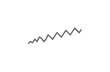
\begin{tikzpicture}[x=0.08em, y=0.08em, line width=0.4pt]
                \draw[FooterGray] (0,3) -- (1,4) -- (2,3.5) -- (3,5) -- (4,4) -- (5,6) -- (6,5.5) -- (7,4) -- (8,5) -- (9,7) -- (10,6) -- (11,5) -- (12,6.5) -- (13,8) -- (14,7) -- (15,6) -- (16,7.5) -- (17,9) -- (18,8) -- (19,7) -- (20,8.5) -- (21,10) -- (22,9) -- (23,8) -- (24,9.5);
            \end{tikzpicture}%
        }%
        \hskip0.5cm%
    }%
    \vskip6pt%
}

%=============================================================================
% PACHETE
%=============================================================================
\usepackage[utf8]{inputenc}
\usepackage[T1]{fontenc}
\usepackage{amsmath, amssymb, amsthm}
\usepackage{mathtools}
\usepackage{bm}
\usepackage{tikz}
\usetikzlibrary{arrows.meta, positioning, shapes, calc, decorations.pathreplacing, shadings}
\usepackage{booktabs}
\usepackage{multirow}
\usepackage{array}
\usepackage{graphicx}
\usepackage{hyperref}
\usepackage{colortbl}
\hypersetup{colorlinks=true, linkcolor=MainBlue, urlcolor=MainBlue}
\graphicspath{{../../logos/}{../../charts/}}
\hfuzz=2pt  % Suppress tiny overfull warnings (<2pt)
\vfuzz=2pt  % Suppress tiny vertical overfull warnings (<2pt)

%=============================================================================
% COMANDA QUANTLET
%=============================================================================
\newcommand{\quantlet}[2]{%
    \hfill\href{#2}{%
        \raisebox{-0.15em}{\includegraphics[height=0.7em]{ql_logo.png}}%
        \textcolor{MainBlue}{\tiny\ #1}%
    }%
}

%=============================================================================
% PAGINĂ TITLU PERSONALIZATĂ
%=============================================================================
\defbeamertemplate*{title page}{hybrid}[1][]
{
    \vspace{0.2cm}
    % Logos row - top header (with clickable links)
    \begin{center}
        \href{https://www.ase.ro}{\includegraphics[height=1.0cm]{ase_logo.png}}\hspace{0.3cm}%
        \href{https://theida.net}{\includegraphics[height=1.0cm]{ida_logo.png}}\hspace{0.3cm}%
        \href{https://blockchain-research-center.com}{\includegraphics[height=1.0cm]{brc_logo.png}}\hspace{0.3cm}%
        \href{https://www.ai4efin.ase.ro}{\includegraphics[height=1.0cm]{ai4efin_logo.png}}\hspace{0.3cm}%
        \href{https://ipe.ro/new}{\includegraphics[height=1.0cm]{acad_logo.png}}\hspace{0.3cm}%
        \href{https://www.digital-finance-msca.com}{\includegraphics[height=1.0cm]{msca_logo.png}}%
    \end{center}

    \vspace{0.6cm}

    % Main title with Q logos on sides (with clickable links)
    \begin{center}
        \begin{minipage}{0.1\textwidth}
            \centering
            \href{https://quantlet.com}{\includegraphics[height=1.1cm]{ql_logo.png}}
        \end{minipage}%
        \begin{minipage}{0.78\textwidth}
            \centering
            {\LARGE\bfseries\usebeamercolor[fg]{title}\inserttitle}

            \vspace{0.3cm}

            {\usebeamerfont{subtitle}\usebeamercolor[fg]{title}\insertsubtitle}
        \end{minipage}%
        \begin{minipage}{0.1\textwidth}
            \centering
            \href{https://quantinar.com}{\includegraphics[height=1.1cm]{qr_logo.png}}
        \end{minipage}
    \end{center}

    \vspace{0.6cm}

    % Authors (left aligned)
    \hspace{0.5cm}{\usebeamerfont{author}\insertauthor}

    \vspace{0.3cm}

    % Institute/Affiliations (left aligned)
    \hspace{0.5cm}\begin{minipage}[t]{0.9\textwidth}
        \raggedright\small\insertinstitute
    \end{minipage}
}

%=============================================================================
% MEDII PENTRU TEOREME
%=============================================================================
\theoremstyle{definition}
\setbeamertemplate{theorems}[numbered]
\newtheorem{defn}{Definiție}
\newtheorem{thm}{Teoremă}
\newtheorem{prop}{Propoziție}
\newtheorem{rmk}{Observație}

%=============================================================================
% COMENZI PERSONALIZATE
%=============================================================================
\newcommand{\E}{\mathbb{E}}
\newcommand{\Var}{\text{Var}}
\newcommand{\Cov}{\text{Cov}}
\newcommand{\Corr}{\text{Corr}}
\newcommand{\R}{\mathbb{R}}
\newcommand{\N}{\mathbb{N}}
\newcommand{\Z}{\mathbb{Z}}
\newcommand{\B}{\mathbf{B}}
\newcommand{\imark}{\textcolor{MainBlue}{\textbullet}}
\newcommand{\RMSE}{\text{RMSE}}
\newcommand{\MAE}{\text{MAE}}
\newcommand{\MAPE}{\text{MAPE}}

%=============================================================================
% INFORMAȚII TITLU
%=============================================================================
\title[Analiza Seriilor de Timp]{Analiza și Prognoza Seriilor de Timp}
\subtitle{Capitolul 9: Prophet și TBATS}
\author[D.T. Pele]{Daniel Traian PELE}
\institute{Academia de Studii Economice din București\\
IDA Institute Digital Assets\\
Blockchain Research Center\\
AI4EFin Artificial Intelligence for Energy Finance\\
Academia Română, Institutul de Prognoză Economică\\
MSCA Digital Finance}
\date{}

\begin{document}

% Title page (no header/footer)
{
\setbeamertemplate{headline}{}
\setbeamertemplate{footline}{}
\begin{frame}
    \titlepage
\end{frame}
}

%=============================================================================
% LEARNING OBJECTIVES
%=============================================================================
\begin{frame}{Obiective de învățare}
    \begin{block}{La finalul acestui capitol, veți fi capabili să:}
        \begin{enumerate}\setlength{\itemsep}{0pt}
            \item Gestionați serii de timp cu \textbf{sezonalități multiple}
            \item Utilizați \textbf{Facebook Prophet} pentru prognoză flexibilă cu sărbători
            \item Aplicați modele \textbf{TBATS} pentru sezonalitate complexă
            \item Comparați și selectați între metodele moderne de prognoză
        \end{enumerate}
    \end{block}
\end{frame}

%=============================================================================
% OUTLINE
%=============================================================================
\begin{frame}{Cuprins}
    \vspace{-0.3cm}
    {\small
    \begin{columns}[T]
        \begin{column}{0.48\textwidth}
            \begin{block}{Fundamente}
                \begin{itemize}\setlength{\itemsep}{3pt}
                    \item Sezonalități Multiple
                    \item Modelul TBATS
                    \item Facebook Prophet
                \end{itemize}
            \end{block}
        \end{column}
        \begin{column}{0.48\textwidth}
            \begin{exampleblock}{Aplicații}
                \begin{itemize}\setlength{\itemsep}{3pt}
                    \item Comparație și Ghid de Selecție
                    \item Studiu de Caz
                    \item Rezumat și Quiz
                \end{itemize}
            \end{exampleblock}
        \end{column}
    \end{columns}
    }
\end{frame}

%=============================================================================
% SECTION 1: MOTIVATION
%=============================================================================
\section{Sezonalități Multiple}

\begin{frame}{Problema: tipare sezoniere complexe}
    \begin{block}{Exemple din Lumea Reală}
        \begin{itemize}\setlength{\itemsep}{0pt}
            \item \textbf{Cerere de electricitate pe oră}: Tipare zilnice + săptămânale + anuale
            \item \textbf{Trafic web}: Zilnic + săptămânal + efecte de sărbători
            \item \textbf{Vânzări retail}: Săptămânal + lunar + anual + sărbători
            \item \textbf{Volum call center}: Pe oră + zilnic + săptămânal
        \end{itemize}
    \end{block}

    \vspace{0.3cm}

    \begin{alertblock}{Limitarea SARIMA}
        \begin{itemize}\setlength{\itemsep}{0pt}
            \item SARIMA$(p,d,q)(P,D,Q)_s$ standard gestionează doar \textbf{o singură} perioadă sezonieră $s$
            \item Pentru date orare cu tipare zilnice ȘI săptămânale, avem nevoie de $s_1 = 24$ și $s_2 = 168$
        \end{itemize}
    \end{alertblock}
\end{frame}

\begin{frame}{Soluții pentru sezonalități multiple}
    \vspace{-0.2cm}
    \begin{columns}[T]
        \column{0.5\textwidth}
        \begin{block}{Abordări Tradiționale}
            \begin{itemize}\setlength{\itemsep}{0pt}
                \item \textbf{Termeni Fourier}: Adăugare regresori sin/cos
                \item \textbf{Variabile dummy}: Mulți parametri
                \item \textbf{Modele nested}: Specificare complexă
            \end{itemize}
        \end{block}

        \column{0.5\textwidth}
        \begin{exampleblock}{Abordări Moderne}
            \begin{itemize}\setlength{\itemsep}{0pt}
                \item \textbf{TBATS}: Automat, gestionează multe perioade
                \item \textbf{Prophet}: Flexibil, interpretabil
                \item \textbf{Metode neurale}: Deep learning
            \end{itemize}
        \end{exampleblock}
    \end{columns}

    \vspace{0.1cm}

    {\footnotesize
    \begin{block}{Comparație}
        \begin{itemize}\setlength{\itemsep}{0pt}
            \item Rezumat comparativ:
        \end{itemize}
        \vspace{-0.2cm}
        \begin{center}
        \begin{tabular}{lcc}
            \toprule
            \textbf{Metodă} & \textbf{Nr. Max Sezonalități} & \textbf{Interpretabil} \\
            \midrule
            SARIMA & 1 & Da \\
            Fourier + ARIMA & Multiple & Moderat \\
            TBATS & Multiple & Moderat \\
            Prophet & Multiple & Da \\
            \bottomrule
        \end{tabular}
        \end{center}
    \end{block}
    }
\end{frame}

\begin{frame}{Exemplu: date orare cu sezonalități multiple}
    \begin{center}
        \includegraphics[width=0.95\textwidth, height=0.70\textheight, keepaspectratio]{ch9_multiple_seasonality.pdf}
    \end{center}
    \quantlet{TSA\_ch9\_multiple\_seasonality}{https://github.com/QuantLet/TSA/tree/main/TSA_ch9/TSA_ch9_multiple_seasonality}
\end{frame}

\begin{frame}{Exemplu real: cerere de electricitate}
    \begin{center}
        \includegraphics[width=0.95\textwidth, height=0.70\textheight, keepaspectratio]{ch9_electricity_demand.pdf}
    \end{center}
    \quantlet{TSA\_ch9\_electricity\_demand}{https://github.com/QuantLet/TSA/tree/main/TSA_ch9/TSA_ch9_electricity_demand}
\end{frame}

\begin{frame}{Exemplu real: vânzări retail cu sărbători}
    \begin{center}
        \includegraphics[width=0.95\textwidth, height=0.70\textheight, keepaspectratio]{ch9_retail_sales.pdf}
    \end{center}
    \quantlet{TSA\_ch9\_retail\_sales}{https://github.com/QuantLet/TSA/tree/main/TSA_ch9/TSA_ch9_retail_sales}
\end{frame}

%=============================================================================
% SECTION 2: TBATS
%=============================================================================
\section{Modelul TBATS}

\begin{frame}{TBATS: ce înseamnă?}
    \begin{block}{Componentele TBATS}
        \begin{itemize}\setlength{\itemsep}{0pt}
            \item \textbf{T} $\succ$ Sezonalitate \textbf{Trigonometrică} folosind termeni Fourier
            \item \textbf{B} $\succ$ Transformare \textbf{Box-Cox} pentru stabilizarea varianței
            \item \textbf{A} $\succ$ Erori \textbf{ARMA} pentru autocorelația reziduală
            \item \textbf{T} $\succ$ Componentă de \textbf{Trend} (posibil amortizat)
            \item \textbf{S} $\succ$ Componente \textbf{Sezoniere} (multiple permise)
        \end{itemize}
    \end{block}

    \vspace{0.1cm}

    \begin{exampleblock}{Inovația Cheie}
        \begin{itemize}\setlength{\itemsep}{0pt}
            \item TBATS folosește \textbf{reprezentare trigonometrică} pentru sezonalitate:
            \[
            s_t^{(i)} = \sum_{j=1}^{k_i} \left[ s_j^{(i)} \cos\left(\frac{2\pi j t}{m_i}\right) + s_j^{*(i)} \sin\left(\frac{2\pi j t}{m_i}\right) \right]
            \]
            \item $m_i$ este perioadă sezonieră $i$ și $k_i$ este numărul de armonici
        \end{itemize}
    \end{exampleblock}
\end{frame}

\begin{frame}{Structura modelului TBATS}
    \vspace{-0.3cm}
    {\small
    \begin{block}{Specificația Completă a modelului}
        \begin{itemize}\setlength{\itemsep}{0pt}
            \item Ecuațiile modelului TBATS:
        {\footnotesize
        \begin{align}
            y_t^{(\omega)} &= \ell_{t-1} + \phi b_{t-1} + \sum_{i=1}^{M} s_t^{(i)} + d_t \\[0.05cm]
            \ell_t &= \ell_{t-1} + \phi b_{t-1} + \alpha d_t \\[0.05cm]
            b_t &= \phi b_{t-1} + \beta d_t \\[0.05cm]
            d_t &= \sum_{i=1}^{p} \varphi_i d_{t-i} + \sum_{j=1}^{q} \theta_j \varepsilon_{t-j} + \varepsilon_t
        \end{align}
        }
        \end{itemize}
    \end{block}
    }

    \vspace{-0.2cm}

    {\scriptsize
    \begin{block}{Notații}
        \begin{itemize}\setlength{\itemsep}{0pt}
            \item $y_t^{(\omega)}$ $\succ$ seria transformată Box-Cox (dacă $\omega \neq 1$)
            \item $\ell_t$ $\succ$ nivelul local, $b_t$ $\succ$ trendul cu amortizare $\phi$
            \item $s_t^{(i)}$ $\succ$ $M$ componente sezoniere cu perioade $m_1, \ldots, m_M$
            \item $d_t$ $\succ$ procesul de eroare ARMA$(p,q)$
        \end{itemize}
    \end{block}
    }
\end{frame}

\begin{frame}{TBATS: sezonalitate trigonometrică}
    \begin{block}{De ce Termeni Fourier/Trigonometrici?}
        \begin{itemize}\setlength{\itemsep}{0pt}
            \item \textbf{Simplu}: Mai puțini parametri decât variabilele dummy
            \item \textbf{Neted}: Captează natural tiparele sezoniere netede
            \item \textbf{Flexibil}: Numărul de armonici $k$ controlează complexitatea
            \item \textbf{Perioade non-întregi}: Poate gestiona $s = 365.25$ pentru date zilnice
        \end{itemize}
    \end{block}

    \vspace{0.3cm}

    \begin{columns}[T]
        \column{0.5\textwidth}
        \begin{exampleblock}{$k$ mic (puține armonici)}
            \begin{itemize}\setlength{\itemsep}{0pt}
                \item Tipar neted
                \item Mai puțini parametri
                \item Poate rata vârfuri abrupte
            \end{itemize}
        \end{exampleblock}

        \column{0.5\textwidth}
        \begin{alertblock}{$k$ mare (multe armonici)}
            \begin{itemize}\setlength{\itemsep}{0pt}
                \item Poate capta orice tipar
                \item Mai mulți parametri
                \item Risc de supraajustare
            \end{itemize}
        \end{alertblock}
    \end{columns}
\end{frame}

\begin{frame}{Aproximarea Fourier a sezonalității}
    \begin{center}
        \includegraphics[width=0.95\textwidth, height=0.70\textheight, keepaspectratio]{ch9_fourier_approximation.pdf}
    \end{center}
    \quantlet{TSA\_ch9\_fourier\_approximation}{https://github.com/QuantLet/TSA/tree/main/TSA_ch9/TSA_ch9_fourier_approximation}
\end{frame}

\begin{frame}{TBATS în practică}
    \vspace{-0.2cm}
    {\small
    \begin{block}{Implementare Python}
        \begin{itemize}\setlength{\itemsep}{0pt}
            \item \textbf{Pachet \texttt{tbats}}: Oferă selecție automată a modelului
            \begin{itemize}\setlength{\itemsep}{0pt}
                \item Selectează automat parametrul Box-Cox $\omega$
                \item Alege numărul de armonici $k_i$ pentru fiecare perioadă sezonieră
                \item Selectează ordinele ARMA $(p,q)$
                \item Testează trend amortizat vs neamortizat
            \end{itemize}
        \end{itemize}
    \end{block}

    \vspace{0.1cm}

    \begin{exampleblock}{Exemplu de Cod}
        \begin{itemize}\setlength{\itemsep}{0pt}
            \item Cod Python:
        \footnotesize
        \texttt{from tbats import TBATS}\\
        \texttt{estimator = TBATS(seasonal\_periods=[7, 365.25])}\\
        \texttt{model = estimator.fit(y)}\\
        \texttt{forecast = model.forecast(steps=30)}
        \end{itemize}
    \end{exampleblock}

    \vspace{0.1cm}

    \begin{alertblock}{Notă}
        \begin{itemize}\setlength{\itemsep}{0pt}
            \item BATS este versiunea mai simplă fără termeni trigonometrici (folosește stări sezoniere tradiționale)
        \end{itemize}
    \end{alertblock}
    }
\end{frame}

\begin{frame}{TBATS: avantaje și limitări}
    \small
    \begin{columns}[T]
        \column{0.5\textwidth}
        \begin{exampleblock}{Avantaje}
            \begin{itemize}\setlength{\itemsep}{0pt}
                \item Gestionează \textbf{multiple} perioade sezoniere
                \item Selecție \textbf{automată} a modelului
                \item Gestionează perioade \textbf{non-întregi} (365.25)
                \item \textbf{Box-Cox} pentru heteroscedasticitate
                \item Bun pentru date de \textbf{frecvență înaltă}
            \end{itemize}
        \end{exampleblock}

        \column{0.5\textwidth}
        \begin{alertblock}{Limitări}
            \begin{itemize}\setlength{\itemsep}{0pt}
                \item \textbf{Intensiv computațional}
                \item Fără \textbf{regresori externi}
                \item Mai puțin \textbf{interpretabil} decât Prophet
                \item Poate fi \textbf{lent} pentru serii foarte lungi
                \item Necesită \textbf{suficiente date} per sezon
            \end{itemize}
        \end{alertblock}
    \end{columns}
\end{frame}

\begin{frame}{Exemplu descompunere TBATS}
    \begin{center}
        \includegraphics[width=0.95\textwidth, height=0.70\textheight, keepaspectratio]{ch9_tbats_decomposition.pdf}
    \end{center}
    \quantlet{TSA\_ch9\_tbats\_decomposition}{https://github.com/QuantLet/TSA/tree/main/TSA_ch9/TSA_ch9_tbats_decomposition}
\end{frame}

%=============================================================================
% SECTION 3: PROPHET
%=============================================================================
\section{Facebook Prophet}

\begin{frame}{Prophet: prezentare generală}
    \begin{block}{Ce este Prophet?}
        \begin{itemize}\setlength{\itemsep}{0pt}
            \item \textbf{Origine}: Procedură de prognoză dezvoltată de Facebook (Meta) în 2017
            \item \textbf{Proiectat pentru serii de timp de business} cu:
            \begin{itemize}\setlength{\itemsep}{0pt}
                \item Efecte sezoniere puternice (zilnice, săptămânale, anuale)
                \item Efecte de sărbători
                \item Schimbări de trend (changepoints)
                \item Date lipsă și outlieri
            \end{itemize}
        \end{itemize}
    \end{block}

    \vspace{0.3cm}

    \begin{exampleblock}{Filosofia Cheie}
        \begin{itemize}\setlength{\itemsep}{0pt}
            \item \textit{``Analyst-in-the-loop'' forecasting}
            \item Prophet este proiectat pentru a fi ajustat de analiști cu cunoștințe de domeniu, dar care nu sunt neapărat experți în serii de timp
        \end{itemize}
    \end{exampleblock}
\end{frame}

\begin{frame}{Structura modelului Prophet}
    \begin{block}{Abordare prin Descompunere}
        \begin{itemize}\setlength{\itemsep}{0pt}
            \item Prophet folosește o \textbf{descompunere aditivă}:
            \[
            y(t) = g(t) + s(t) + h(t) + \varepsilon_t
            \]
        \end{itemize}
    \end{block}

    \vspace{0.3cm}

    \begin{columns}[T]
        \column{0.33\textwidth}
        \begin{block}{$g(t)$: Trend}
            \begin{itemize}\setlength{\itemsep}{0pt}
                \item Liniar sau logistic
                \item Changepoints automate
                \item Saturație de creștere
            \end{itemize}
        \end{block}

        \column{0.33\textwidth}
        \begin{block}{$s(t)$: Sezonalitate}
            \begin{itemize}\setlength{\itemsep}{0pt}
                \item Serii Fourier
                \item Perioade multiple
                \item Sezonalitate custom
            \end{itemize}
        \end{block}

        \column{0.33\textwidth}
        \begin{block}{$h(t)$: Sărbători}
            \begin{itemize}\setlength{\itemsep}{0pt}
                \item Sărbători pe țară
                \item Evenimente custom
                \item Efecte de fereastră
            \end{itemize}
        \end{block}
    \end{columns}
\end{frame}

\begin{frame}{Prophet: componenta de trend}
    \vspace{-0.2cm}
    {\small
    \begin{block}{Trend Liniar cu Changepoints}
        \begin{itemize}\setlength{\itemsep}{0pt}
            \item \textbf{Ecuația}: $g(t) = (k + \bm{a}(t)^T \bm{\delta}) \cdot t + (m + \bm{a}(t)^T \bm{\gamma})$
            \item \textbf{Parametri}:
            \begin{itemize}\setlength{\itemsep}{0pt}
                \item $k$ $\succ$ rata de creștere de bază
                \item $\bm{\delta}$ $\succ$ vector de ajustări de rată la changepoints
                \item $\bm{a}(t)$ $\succ$ indică ce changepoints sunt active la momentul $t$
                \item $m$ $\succ$ offset-ul, $\bm{\gamma}$ asigură continuitatea
            \end{itemize}
        \end{itemize}
    \end{block}
    }

    \vspace{-0.1cm}

    {\footnotesize
    \begin{exampleblock}{Creștere Logistică (pentru trenduri cu saturație)}
        \begin{itemize}\setlength{\itemsep}{0pt}
            \item Ecuația de creștere logistică:
            \[
            g(t) = \frac{C(t)}{1 + \exp(-(k + \bm{a}(t)^T \bm{\delta})(t - (m + \bm{a}(t)^T \bm{\gamma})))}
            \]
            \item $C(t)$ este capacitatea maximă (posibil variabilă în timp)
        \end{itemize}
    \end{exampleblock}
    }
\end{frame}

\begin{frame}{Prophet: componenta de sezonalitate}
    \vspace{-0.3cm}
    {\small
    \begin{block}{Reprezentare prin Serii Fourier}
        \begin{itemize}\setlength{\itemsep}{0pt}
            \item Pentru o perioadă sezonieră $P$, Prophet folosește:
            \vspace{-0.1cm}
            \[
            s(t) = \sum_{n=1}^{N} \left[ a_n \cos\!\left(\frac{2\pi n t}{P}\right) + b_n \sin\!\left(\frac{2\pi n t}{P}\right) \right]
            \]
            \vspace{-0.3cm}
        \end{itemize}
    \end{block}

    \vspace{-0.1cm}

    \begin{exampleblock}{Setări Implicite}
        \begin{itemize}\setlength{\itemsep}{0pt}
            \item \textbf{Anuală}: perioadă 365.25 zile, ordin Fourier 10
            \item \textbf{Săptămânală}: perioadă 7 zile, ordin Fourier 3
            \item \textbf{Zilnică}: perioadă 1 zi, ordin Fourier 4
        \end{itemize}
    \end{exampleblock}

    \vspace{-0.1cm}

    \begin{alertblock}{Atenție}
        \begin{itemize}\setlength{\itemsep}{0pt}
            \item Ordin Fourier $N$ mai mare $\succ$ mai multă flexibilitate (tipare mai complexe) dar risc mai mare de supraajustare
        \end{itemize}
    \end{alertblock}
    }
\end{frame}

\begin{frame}{Descompunerea componentelor Prophet}
    \begin{center}
        \includegraphics[width=0.95\textwidth, height=0.70\textheight, keepaspectratio]{ch9_prophet_components.pdf}
    \end{center}
    \quantlet{TSA\_ch9\_prophet\_components}{https://github.com/QuantLet/TSA/tree/main/TSA_ch9/TSA_ch9_prophet_components}
\end{frame}

\begin{frame}{Detectarea changepoints în trend}
    \begin{center}
        \includegraphics[width=0.95\textwidth, height=0.70\textheight, keepaspectratio]{ch9_changepoint_detection.pdf}
    \end{center}
    \quantlet{TSA\_ch9\_changepoint\_detection}{https://github.com/QuantLet/TSA/tree/main/TSA_ch9/TSA_ch9_changepoint_detection}
\end{frame}

\begin{frame}{Prophet: efecte de sărbători}
    \vspace{-0.15cm}
    \begin{block}{Modelul de Sărbători}
        \begin{itemize}\setlength{\itemsep}{0pt}
            \item Ecuația efectelor de sărbătoare:
            \[
            h(t) = Z(t) \cdot \bm{\kappa}
            \]
            \item $Z(t)$ este o matrice indicător pentru sărbători și $\bm{\kappa}$ sunt efectele sărbătorilor
        \end{itemize}
    \end{block}

    \vspace{0.1cm}

    \begin{exampleblock}{Caracteristici}
        \begin{itemize}\setlength{\itemsep}{0pt}
            \item \textbf{Sărbători integrate}: 60+ țări suportate
            \item \textbf{Sărbători custom}: Adăugați propriile evenimente (Black Friday, evenimente companie)
            \item \textbf{Efecte de fereastră}: Sărbătorile pot afecta zilele înainte/după
            \item \textbf{Prior scale}: Controlează regularizarea efectelor de sărbătoare
        \end{itemize}
    \end{exampleblock}

    \begin{block}{Exemplu de Cod}
        \begin{itemize}\setlength{\itemsep}{0pt}
            \item Cod Python:
        \footnotesize
        \texttt{holidays = pd.DataFrame(\{'holiday': 'black\_friday', ....\})}\\
        \texttt{model = Prophet(holidays=holidays)}
        \end{itemize}
    \end{block}
\end{frame}

\begin{frame}{Prophet în practică}
    \begin{block}{Utilizare de Bază}
        \begin{itemize}\setlength{\itemsep}{0pt}
            \item Cod Python:
        \small
        \texttt{from prophet import Prophet}\\
        \texttt{import pandas as pd}\\[0.2cm]
        \texttt{\# Datele trebuie să aibă coloane 'ds' (dată) și 'y' (valoare)}\\
        \texttt{df = pd.DataFrame(\{'ds': dates, 'y': values\})}\\[0.2cm]
        \texttt{model = Prophet()}\\
        \texttt{model.fit(df)}\\[0.2cm]
        \texttt{future = model.make\_future\_dataframe(periods=365)}\\
        \texttt{forecast = model.predict(future)}
        \end{itemize}
    \end{block}

    \vspace{0.3cm}

    \begin{exampleblock}{Adăugare Sezonalitate Custom}
        \begin{itemize}\setlength{\itemsep}{0pt}
            \item Cod Python:
        \small
        \texttt{model = Prophet(weekly\_seasonality=False)}\\
        \texttt{model.add\_seasonality(name='monthly', period=30.5, fourier\_order=5)}\\
        \texttt{model.add\_seasonality(name='quarterly', period=91.25, fourier\_order=3)}
        \end{itemize}
    \end{exampleblock}
\end{frame}

\begin{frame}{Prophet: cuantificarea incertitudinii}
    \begin{block}{Trei Surse de Incertitudine}
        \begin{itemize}\setlength{\itemsep}{0pt}
            \item \textbf{Incertitudine de trend}: Changepoints viitoare sunt incerte
            \item \textbf{Incertitudine de sezonalitate}: Incertitudine în estimarea parametrilor
            \item \textbf{Zgomot de observație}: Aleatorietate inerentă
        \end{itemize}
    \end{block}

    \vspace{0.3cm}

    \begin{columns}[T]
        \column{0.6\textwidth}
        \begin{exampleblock}{Intervale de Predicție}
            \begin{itemize}\setlength{\itemsep}{0pt}
                \item \textbf{Prophet oferă}:
                \begin{itemize}\setlength{\itemsep}{0pt}
                    \item Prognoză punctuală: \texttt{yhat}
                    \item Limita inferioară: \texttt{yhat\_lower}
                    \item Limita superioară: \texttt{yhat\_upper}
                \end{itemize}
                \item \textbf{Implicit}: interval de 80\%, schimbați cu \texttt{interval\_width=0.95}
            \end{itemize}
        \end{exampleblock}

        \column{0.4\textwidth}
        \begin{alertblock}{Notă}
            \begin{itemize}\setlength{\itemsep}{0pt}
                \item Incertitudinea crește cu orizontul de prognoză, în special pentru incertitudinea de trend
            \end{itemize}
        \end{alertblock}
    \end{columns}
\end{frame}

\begin{frame}{Prophet: parametri de ajustare}
    \begin{block}{Parametri Cheie}
        \begin{itemize}\setlength{\itemsep}{0pt}
            \item \textbf{\texttt{changepoint\_prior\_scale}}: Flexibilitate trend (implicit: 0.05)
            \item \textbf{\texttt{seasonality\_prior\_scale}}: Flexibilitate sezonalitate (implicit: 10)
            \item \textbf{\texttt{holidays\_prior\_scale}}: Mărime efect sărbători (implicit: 10)
            \item \textbf{\texttt{seasonality\_mode}}: 'additive' sau 'multiplicative'
            \item \textbf{\texttt{changepoint\_range}}: Porțiune din istoric pentru changepoints
        \end{itemize}
    \end{block}

    \vspace{0.3cm}

    \begin{exampleblock}{Sfaturi Practice}
        \begin{itemize}\setlength{\itemsep}{0pt}
            \item \textbf{Supraajustare pe trend?} Micșorați \texttt{changepoint\_prior\_scale}
            \item \textbf{Subajustare pe sezonalitate?} Măriți \texttt{seasonality\_prior\_scale}
            \item \textbf{Amplitudinea sezonieră variază?} Folosiți \texttt{seasonality\_mode='multiplicative'}
        \end{itemize}
    \end{exampleblock}
\end{frame}

\begin{frame}{Prophet: avantaje și limitări}
    \small
    \begin{columns}[T]
        \column{0.5\textwidth}
        \begin{exampleblock}{Avantaje}
            \begin{itemize}\setlength{\itemsep}{0pt}
                \item \textbf{Ușor de folosit}: Ajustare minimă necesară
                \item \textbf{Interpretabil}: Descompunere clară
                \item \textbf{Gestionează date lipsă} bine
                \item \textbf{Efecte sărbători} integrate
                \item \textbf{Sezonalități multiple}
                \item \textbf{Regresori externi} suportați
                \item \textbf{Ajustare rapidă}
            \end{itemize}
        \end{exampleblock}

        \column{0.5\textwidth}
        \begin{alertblock}{Limitări}
            \begin{itemize}\setlength{\itemsep}{0pt}
                \item \textbf{Nu bazat pe ARIMA}: Fără modelare autocorelație
                \item \textbf{Focus pe date zilnice}: Mai puțin potrivit pentru frecvență foarte înaltă
                \item \textbf{Ipoteze de trend}: Liniar/logistic poate să nu se potrivească
                \item \textbf{CV integrat}: \texttt{cross\_validation()} disponibil, dar necesită configurare atentă
                \item \textbf{Risc supraajustare} cu multe sezonalități
            \end{itemize}
        \end{alertblock}
    \end{columns}
\end{frame}

\begin{frame}{Sezonalitate aditivă vs multiplicativă}
    \begin{center}
        \includegraphics[width=0.95\textwidth, height=0.70\textheight, keepaspectratio]{ch9_additive_vs_multiplicative.pdf}
    \end{center}
    \quantlet{TSA\_ch9\_additive\_vs\_multiplicative}{https://github.com/QuantLet/TSA/tree/main/TSA_ch9/TSA_ch9_additive_vs_multiplicative}
\end{frame}

%=============================================================================
% SECTION 4: COMPARISON
%=============================================================================
\section{Comparație și Ghid de Selecție}

\begin{frame}{TBATS vs Prophet: comparație directă}
    \vspace{-0.2cm}
    \begin{block}{Comparație detaliată}
        \begin{itemize}\setlength{\itemsep}{0pt}
            \item Rezumat al diferențelor cheie:
        \end{itemize}
        \vspace{-0.2cm}
        {\small
        \begin{center}
        \begin{tabular}{p{3.8cm}p{4.2cm}p{4.2cm}}
            \toprule
            \textbf{Caracteristică} & \textbf{TBATS} & \textbf{Prophet} \\
            \midrule
            Sezonalități multiple & Da (automat) & Da (manual sau auto) \\
            Efecte sărbători & Nu & Da (integrat) \\
            Regresori externi & Nu & Da \\
            Changepoints trend & Nu (neted) & Da (automat) \\
            Date lipsă & Necesită interpolare & Gestionează nativ \\
            Interpretabilitate & Moderată & Înaltă \\
            Viteză calcul & Lent & Rapid \\
            Date frecvență înaltă & Bun & Moderat \\
            Perioade non-întregi & Da (ex: 365.25) & Da \\
            Intervale incertitudine & Da & Da \\
            \bottomrule
        \end{tabular}
        \end{center}
        }
    \end{block}
\end{frame}

\begin{frame}{Comparație Prophet vs TBATS: prognoze}
    \begin{center}
        \includegraphics[width=0.95\textwidth, height=0.70\textheight, keepaspectratio]{ch9_prophet_vs_tbats.pdf}
    \end{center}
    \quantlet{TSA\_ch9\_prophet\_vs\_tbats}{https://github.com/QuantLet/TSA/tree/main/TSA_ch9/TSA_ch9_prophet_vs_tbats}
\end{frame}

\begin{frame}{Când să folosim fiecare model}
    \begin{columns}[T]
        \column{0.5\textwidth}
        \begin{block}{Folosiți TBATS când:}
            \begin{itemize}\setlength{\itemsep}{0pt}
                \item Date de frecvență înaltă (orare, sub-zilnice)
                \item Multiple perioade sezoniere complexe
                \item Nu sunt necesari regresori externi
                \item Se preferă selecție automată a modelului
                \item Se dorește framework tradițional state-space
            \end{itemize}
        \end{block}

        \column{0.5\textwidth}
        \begin{block}{Folosiți Prophet când:}
            \begin{itemize}\setlength{\itemsep}{0pt}
                \item Prognoză de business (zilnic/săptămânal)
                \item Efectele sărbătorilor sunt importante
                \item Trendul are rupturi structurale
                \item Sunt prezente date lipsă
                \item Interpretabilitatea este cheie
                \item Sunt disponibili regresori externi
            \end{itemize}
        \end{block}
    \end{columns}

    \vspace{0.5cm}

    \begin{exampleblock}{Ghid General}
        \begin{itemize}\setlength{\itemsep}{0pt}
            \item \textbf{Prophet}: pentru aplicații de business cu date zilnice
            \item \textbf{TBATS}: pentru aplicații tehnice cu date de frecvență înaltă
        \end{itemize}
    \end{exampleblock}
\end{frame}

\begin{frame}{Ghid selecție model}
    \begin{center}
        \includegraphics[width=0.90\textwidth, height=0.60\textheight, keepaspectratio]{ch9_model_selection_guide.pdf}
    \end{center}
    \quantlet{TSA\_ch9\_model\_selection\_guide}{https://github.com/QuantLet/TSA/tree/main/TSA_ch9/TSA_ch9_model_selection_guide}
\end{frame}

\begin{frame}{Diagramă de decizie}
    \vspace{-0.2cm}
    \begin{center}
    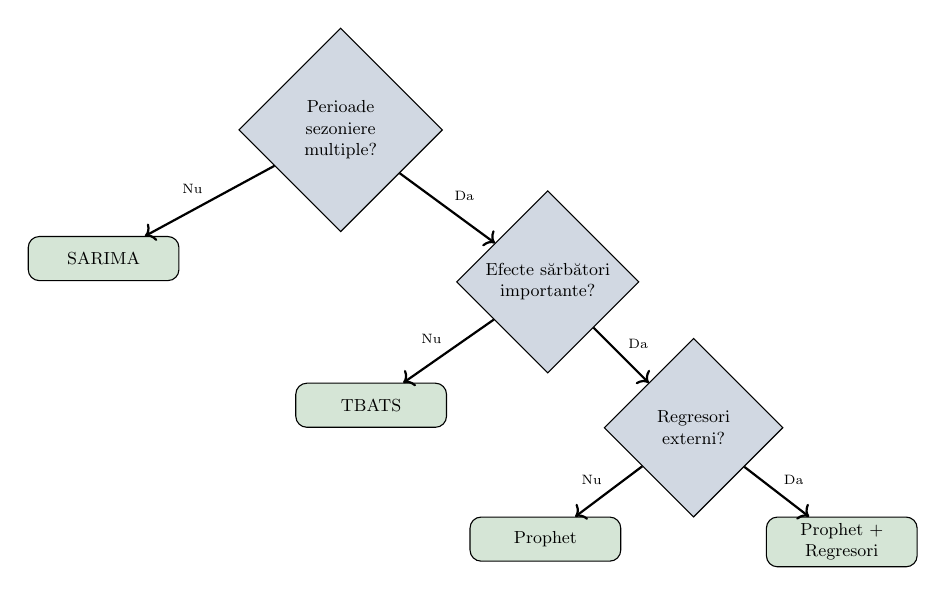
\begin{tikzpicture}[
        scale=0.70, transform shape,
        node distance=1.0cm,
        decision/.style={diamond, draw, fill=MainBlue!20, text width=2.5cm, text centered, inner sep=1pt, font=\small},
        block/.style={rectangle, draw, fill=Forest!20, text width=2.5cm, text centered, rounded corners, minimum height=0.8cm, font=\small},
        line/.style={draw, ->, thick}
    ]
        \node [decision] (q1) {Perioade sezoniere multiple?};
        \node [block, below left=1cm and 2cm of q1] (sarima) {SARIMA};
        \node [decision, below right=1cm and 2cm of q1] (q2) {Efecte sărbători importante?};
        \node [block, below left=1cm and 1cm of q2] (tbats) {TBATS};
        \node [decision, below right=1cm and 1cm of q2] (q3) {Regresori externi?};
        \node [block, below left=0.8cm and 0.5cm of q3] (prophet1) {Prophet};
        \node [block, below right=0.8cm and 0.5cm of q3] (prophet2) {Prophet + Regresori};

        \path [line] (q1) -- node[above left, font=\scriptsize] {Nu} (sarima);
        \path [line] (q1) -- node[above right, font=\scriptsize] {Da} (q2);
        \path [line] (q2) -- node[above left, font=\scriptsize] {Nu} (tbats);
        \path [line] (q2) -- node[above right, font=\scriptsize] {Da} (q3);
        \path [line] (q3) -- node[above left, font=\scriptsize] {Nu} (prophet1);
        \path [line] (q3) -- node[above right, font=\scriptsize] {Da} (prophet2);
    \end{tikzpicture}
    \end{center}
\end{frame}

%=============================================================================
% SECTION 5: PRACTICAL EXAMPLE
%=============================================================================
\section{Studiu de Caz}

\begin{frame}{Studiu de caz: prognoza cererii de energie}
    \begin{block}{Problema}
        \begin{itemize}\setlength{\itemsep}{0pt}
            \item \textbf{Obiectiv}: Prognozați cererea de electricitate pe oră
            \item \textbf{Provocări}:
            \begin{itemize}\setlength{\itemsep}{0pt}
                \item Tipar zilnic $\succ$ vârf la prânz și seara
                \item Tipar săptămânal $\succ$ mai scăzut în weekend
                \item Tipar anual $\succ$ mai mare vara (AC) și iarna (încălzire)
                \item Efecte sărbători $\succ$ cerere mai mică în sărbători
            \end{itemize}
        \end{itemize}
    \end{block}

    \vspace{0.3cm}

    \begin{exampleblock}{Abordare}
        \begin{itemize}\setlength{\itemsep}{0pt}
            \item \textbf{Pas 1}: Încercați TBATS cu perioade [24, 168, 8766]
            \item \textbf{Pas 2}: Încercați Prophet cu sezonalitate zilnică, săptămânală, anuală + sărbători
            \item \textbf{Pas 3}: Comparați folosind cross-validation
        \end{itemize}
    \end{exampleblock}
\end{frame}

\begin{frame}{Studiu de caz: interpretarea rezultatelor}
    \vspace{-0.3cm}
    {\footnotesize
    \begin{block}{Metrici de Evaluare}
        \begin{itemize}\setlength{\itemsep}{0pt}
            \item \textbf{MAPE}: Mean Absolute Percentage Error
            \item \textbf{RMSE}: Root Mean Square Error
            \item \textbf{Acoperire}: \% din valori reale în intervalul de predicție
        \end{itemize}
    \end{block}

    \vspace{0.05cm}

    \begin{exampleblock}{Rezultate Tipice}
        \begin{itemize}\setlength{\itemsep}{0pt}
            \item Comparație performanță:
        \end{itemize}
        \vspace{-0.2cm}
        \begin{center}
        \begin{tabular}{lccc}
            \toprule
            \textbf{Model} & \textbf{MAPE} & \textbf{RMSE} & \textbf{Acoperire} \\
            \midrule
            SARIMA (doar zilnic) & 8.5\% & 450 MW & 75\% \\
            TBATS & 4.2\% & 220 MW & 82\% \\
            Prophet & 4.8\% & 250 MW & 85\% \\
            Prophet + sărbători & 3.9\% & 200 MW & 88\% \\
            \bottomrule
        \end{tabular}
        \end{center}
    \end{exampleblock}

    \vspace{-0.1cm}

    \begin{alertblock}{Concluzie}
        \begin{itemize}\setlength{\itemsep}{0pt}
            \item Modelele cu sezonalități multiple depășesc semnificativ SARIMA cu o singură sezonalitate
        \end{itemize}
    \end{alertblock}
    }
\end{frame}

%=============================================================================
% SECTION 6: SUMMARY
%=============================================================================
\section{Rezumat}

\begin{frame}{Concluzii cheie}
    \begin{block}{Sezonalități Multiple}
        \begin{itemize}\setlength{\itemsep}{0pt}
            \item Datele din lumea reală au adesea tipare sezoniere multiple
            \item SARIMA standard gestionează doar o perioadă sezonieră
            \item TBATS și Prophet sunt proiectate pentru această provocare
        \end{itemize}
    \end{block}

    \vspace{0.3cm}

    \begin{exampleblock}{Selecția modelului}
        \begin{itemize}\setlength{\itemsep}{0pt}
            \item \textbf{TBATS}: Automat, gestionează frecvență înaltă, fără regresori externi
            \item \textbf{Prophet}: Interpretabil, efecte sărbători, regresori externi
            \item Ambele folosesc termeni Fourier pentru reprezentare eficientă a sezonalității
        \end{itemize}
    \end{exampleblock}

    \vspace{0.3cm}

    \begin{alertblock}{De Reținut}
        \begin{itemize}\setlength{\itemsep}{0pt}
            \item \textbf{Validare}: Folosiți întotdeauna cross-validation adecvat pentru serii de timp!
        \end{itemize}
    \end{alertblock}
\end{frame}

\begin{frame}{Întrebări?}
    \vspace{0.5cm}
    \begin{center}
        \Large\textcolor{MainBlue}{Întrebări?}
    \end{center}

    \vspace{0.5cm}

    \begin{exampleblock}{Pași Următori}
        \begin{itemize}\setlength{\itemsep}{0pt}
            \item Exersați cu notebook-ul Jupyter
            \item Încercați Prophet pe propriile date
            \item Explorați NeuralProphet pentru extensia deep learning
        \end{itemize}
    \end{exampleblock}
\end{frame}


%=============================================================================
% QUIZ
%=============================================================================
\section{Quiz}

\begin{frame}{Quiz rapid}
    \begin{block}{Întrebări}
        \begin{itemize}\setlength{\itemsep}{3pt}
            \item \textbf{Q1}: Ce sunt sezonalitățile multiple și de ce SARIMA standard nu le poate gestiona?
            \item \textbf{Q2}: Cum aproximează termenii Fourier o componentă sezonieră?
            \item \textbf{Q3}: Ce reprezintă acronimul TBATS?
            \item \textbf{Q4}: Ce sunt \textit{changepoints} în modelul Prophet?
            \item \textbf{Q5}: Când alegeți Prophet în loc de TBATS (și invers)?
        \end{itemize}
    \end{block}
\end{frame}

\begin{frame}{Răspunsuri quiz}
    {\small
    \begin{block}{Răspunsuri}
        \begin{itemize}\setlength{\itemsep}{2pt}
            \item \textbf{R1}: O serie prezintă mai multe cicluri periodice suprapuse (ex: zilnic + săptămânal + anual). SARIMA acceptă doar o singură perioadă sezonieră $s$
            \item \textbf{R2}: Aproximează sezonalitatea prin combinații de $\sin(2\pi k t / s)$ și $\cos(2\pi k t / s)$. Cu $K$ armonici se captează forme complexe fără a estima un coeficient pentru fiecare perioadă
            \item \textbf{R3}: \textbf{T}rigonometric seasonality, \textbf{B}ox-Cox transformation, \textbf{A}RMA errors, \textbf{T}rend, \textbf{S}easonal components
            \item \textbf{R4}: Puncte în timp unde rata de creștere a trendului se modifică brusc. Prophet le detectează automat prin parametrul \texttt{changepoint\_prior\_scale}
            \item \textbf{R5}: Prophet $\succ$ regresori externi, efecte de sărbători, date lipsă sau rupturi structurale. TBATS $\succ$ frecvență foarte înaltă sau abordare complet automată fără intervenție manuală
        \end{itemize}
    \end{block}
    }
\end{frame}

%=============================================================================
% BIBLIOGRAFIE
%=============================================================================
\begin{frame}{Bibliografie I}
    \begin{block}{Prophet}
        {\small
        \begin{itemize}\setlength{\itemsep}{0pt}
            \item Taylor, S.J., \& Letham, B. (2018). Forecasting at Scale, \textit{The American Statistician}, 72(1), 37--45.
            \item Harvey, A.C. (1989). \textit{Forecasting, Structural Time Series Models and the Kalman Filter}, Cambridge University Press.
        \end{itemize}
        }
    \end{block}

    \begin{exampleblock}{TBATS și netezire exponențială}
        {\small
        \begin{itemize}\setlength{\itemsep}{0pt}
            \item De Livera, A.M., Hyndman, R.J., \& Snyder, R.D. (2011). Forecasting Time Series with Complex Seasonal Patterns Using Exponential Smoothing, \textit{JASA}, 106(496), 1513--1527.
            \item Hyndman, R.J., Koehler, A.B., Ord, J.K., \& Snyder, R.D. (2008). \textit{Forecasting with Exponential Smoothing: The State Space Approach}, Springer.
            \item Taylor, J.W. (2003). Short-term Electricity Demand Forecasting Using Double Seasonal Exponential Smoothing, \textit{Journal of the Operational Research Society}, 54(8), 799--805.
        \end{itemize}
        }
    \end{exampleblock}
\end{frame}

\begin{frame}{Bibliografie II}
    \begin{block}{Comparații și competiții de prognoză}
        {\small
        \begin{itemize}\setlength{\itemsep}{0pt}
            \item Makridakis, S., Spiliotis, E., \& Assimakopoulos, V. (2020). The M4 Competition, \textit{International Journal of Forecasting}, 36(1), 54--74.
            \item Hyndman, R.J., \& Athanasopoulos, G. (2021). \textit{Forecasting: Principles and Practice}, 3rd ed., OTexts.
            \item Petropoulos, F., et al. (2022). Forecasting: Theory and Practice, \textit{International Journal of Forecasting}, 38(3), 845--1054.
        \end{itemize}
        }
    \end{block}

    \begin{exampleblock}{Resurse online și cod}
        {\small
        \begin{itemize}\setlength{\itemsep}{0pt}
            \item \textbf{Quantlet}: \url{https://quantlet.com} $\succ$ Depozit de cod pentru statistică
            \item \textbf{Quantinar}: \url{https://quantinar.com} $\succ$ Platformă de învățare metode cantitative
            \item \textbf{GitHub TSA}: \url{https://github.com/QuantLet/TSA} $\succ$ Cod Python pentru acest curs
        \end{itemize}
        }
    \end{exampleblock}
\end{frame}

\begin{frame}{}
    \centering
    \Huge\textcolor{MainBlue}{Vă Mulțumim!}

    \vspace{1cm}

    \Large Întrebări?

    \vspace{0.8cm}

    \normalsize

    Materialele cursului sunt disponibile la: \url{https://danpele.github.io/Time-Series-Analysis/}

    \vspace{0.2cm}

    \href{https://quantlet.com}{\raisebox{-0.15em}{\includegraphics[height=0.8em]{ql_logo.png}} Quantlet} \hspace{0.5cm}
    \href{https://quantinar.com}{\raisebox{-0.15em}{\includegraphics[height=0.8em]{qr_logo.png}} Quantinar}
\end{frame}

\end{document}
